
\chapter{Results}

In this chapter, I will talk more about the implementation details of the \gls{fids}. I will also look into the security of this implementation and what measures can be implemented to improve it. 

\section{System Architecture}
\label{sec:Architecture}

\begin{figure}[ht]
	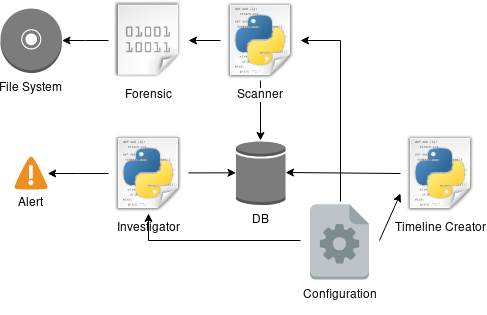
\includegraphics[width=8cm]{../img/Overview_FIDS.png}
	\centering
	\caption{System Architecture}
	\label{fig:systemArchitecture}
\end{figure}

As seen in figure \ref{fig:systemArchitecture}, the \gls{fids} contains two main components, the scanner and the investigator, a database and has connections to some libraries. It is split into scanner and investigator way to gain flexibility, mainly so that both components can be executed independently. This independence has the advantage that the scanner and the investigator don't need to be run on the same system. Also, it means that previous results of the investigator can be recreated by running the investigator on previously captured data. Additionally, if someone is only interested in the results of the scanner, the investigator doesn't need to be run. The scanner is explained in detail in section \ref{sec:Scanner} and the investigator in section \ref{sec:Investigator}.

Besides the scanner and the investigator which were produced in this thesis, there are five other components which build the environment of the \gls{hids}. There is the \gls{fs} which contains the data in which we are interested. As already mentioned, this could be a mounted device that is directly accessible through the operating system. It could also be run on the disk images of virtual machines or previously created disk images. To run it on a previously created disk image might be interesting if used on backup images if backups are made by creating disk images. 

Then there is the forensic component. This component is the combination of \gls{tsk} and \gls{pytsk}. The main purpose of this component is the abstraction of the \gls{fs} into python classes, which can then be used within the scanner. This abstraction is important to be compatible with multiple different \glspl{fs}. \gls{tsk} offers much different functionality; the \gls{fids} is only using the utility that is used for the fls command described in section \ref{sec:fls}. 

This leaves the configuration and the database. Both of which are also part of this thesis. The database is used to store the data of each run, and the configuration is used to change the behavior of the \gls{fids}. The configuration is explained in depth in section \ref{sec:Configuration} and the database in section \ref{sec:Database}.

There is another component that is not part of the \gls{hids} functionality. The \gls{fids} contains a component that is used to create a timeline. This component is special because it is designed for use by forensic investigators. It is explained in section \ref{sec:Timeliner}.

\subsection{Configuration}
\label{sec:Configuration}

The configuration file is provided in \gls{yaml}. \gls{yaml} is a human-friendly data serialization language with support for many programming languages. Its main advantage over other languages for configuration files is the readability and the ease to extend already existing configuration files. There were more reasons why \gls{yaml} is used documented in appendix section \ref{sec:decisions:config:language}.

\subsubsection{Database Configuration}

The configuration consists of three parts. The first part is the database configuration. The current implementation supports only \gls{sqlite}, as this is the most basic and easy to use format. Additionally, it doesn't require any connection to an external entity. For more information on why \gls{sqlite} was chosen see appendix section \ref{sec:decisions:dbms}. For the configuration, only the filename is required as seen in listing \ref{lst:cfg:sqlite}. This configuration defines where the data will be sent to and read from in the scanner and investigator parts, respectively. As both parts need access to the database, this part of the configuration is in a separate part. It is possible and already prepared to extend the system to use more \gls{dbms}. However, this is not part of the scope of this thesis.

\begin{lstlisting}[language=yaml, numbers=left, caption=SQLite Configuration, label=lst:cfg:sqlite]
sqlite:
	filename: fids_db3.db
\end{lstlisting}

\subsubsection{Scanner Configuration}

The second part of the configuration is the part that defines the scanner. An example config can be seen in listing \ref{lst:cfg:scanner}. It consists of one main key, which is named scan. If this config entry is missing, the scanner part of the \gls{hids} is not executed by default. Beneath this top key it contains the following subkeys:

\begin{description}
	\item [image\_path] Path to the \gls{fs} that is used for the scan.
	\item [scan\_paths] List of paths to scan. Paths are scanned recursively. "/" thus scans all available paths.
	\item [ignore\_paths] Paths that should not be scanned. Can be any directory. The recursion stops once this path is reached and does not continue downwards. Practical if certain directories are not interesting for intrusion detection.
\end{description}

\begin{lstlisting}[language=yaml, numbers=left, caption=Scanner Configuration, label=lst:cfg:scanner]
scan:
	image_path: /dev/nvme0n1p1
	scan_paths: 
		[
			"/",
			"/nonExisting",
		]
	ignore_paths: 
		[
			"/temp/"
		]
\end{lstlisting}

\subsubsection{Investigator Configuration}
\label{sec:conf:investigator}

The investigator configuration is similar to the scanner configuration in the way that it contains a top-level node called investigator. If this is missing the investigator part does not start. As can be seen in listing \ref{lst:cfg:investigator} it is a lot more complicated than the scanner configuration. 

\begin{description}
    \item [same\_config] This configuration specifies whether a changed config should result in an alert. Defaults to True.
    \item [validation\_run] This can define a run that is used for validation. If empty the second last one will automatically be used.
    \item [\nameref{sec:config:rules}] Rules are ways to create templates on how changed files should be found. \nameref{sec:config:rules} are explained more through below.
    \item [\nameref{sec:config:investigations}] Investigations define which paths and which files should be checked for intrusions. \nameref{sec:config:investigations} are explained more through below.
\end{description}

\begin{lstlisting}[language=yaml, numbers=left, caption=Investigator Configuration, label=lst:cfg:investigator]
investigator:
	same_config: True
	validation_run: 
	rules: 
		- name: php
		  rules: 
			- m
			- i
			- l
			- n
			- a
		  equal:
			- meta_creation_time
			- meta_size
		- name: logs
		  greater:
			- meta_size
		  equal:
			- meta_creation_time
	investigations:
		- paths:
			- '/etc'
		  fileregexwhitelist:
			- '*.php'
		  rules:
			- php
		- fileregexwhitelist: '/*'
		  fileregexblacklist: '*evilfile*'
		  rules:
			- logs
\end{lstlisting}

\subsubsection{Rules}
\label{sec:config:rules}

Rules represent templates that are later used in the investigations to find anomalies. Rules can be based upon other rules to extend them. Recursive rules are allowed, they simply extend each other. An example of the rule configuration can be seen in listing \ref{lst:cfg:investigator}, the fields are explained below.

\begin{description}
	\item [name] Each rule has a name. If two rules with the same name are defined, the behavior might be inconsistent. The name is used to extend rules.
	\item [rules] The rules which are used as a basis for this rule. They are referenced by name.
	\item [greater] The properties which are allowed to grow between the runs. Greater also includes equal.
	\item [equal] The properties that are supposed to stay equal during all runs.
\end{description}

Additionally, there are some predefined rules. The aide configuration heavily influenced which rules got predefined. The preconfigured rules are listed in listing \ref{lst:cfg:precon}.
\begin{lstlisting}[language=yaml, numbers=left, caption=Preconfigured Rules, label=lst:cfg:precon]
rules: 
	- name: p
	  equal:
		- meta_mode
	- name: ftype
	  equal:
		- meta_conten
	- name: i
	  equal:
		- meta_addr
	- name: l
	  equal:
		- meta_link
	- name: n
	  equal:
		- meta_nlink 
	- name: g
	  equal:
		- meta_gid
	- name: s
	  equal:
		- meta_size
	- name: m
	  equal:
		- meta_modification_time
		- meta_modification_time_nano
	- name: a
	  equal:
		- meta_access_time
		- meta_access_time_nano
	- name: c
	  equal:
		- meta_changed_time
		- meta_changed_time_nano
	- name: S
	  greater:
		- meta_size
\end{lstlisting}
	
Additional to those, there are some rules which do not directly check the \gls{fs} \gls{metadata}. There are three of them which change the behavior of the investigator. They must be configured on the investigation level. They are directly referenced by the investigator to specify if the related events should result in an alert or not. 

\begin{description}
    \item [file\_rename\_ok]    Usually a changed filename leads to an alert. This behavior is deactivated by setting this rule.
    \item [new\_files\_ok]    Usually a new file leads to an alert. This behavior is deactivated by setting this rule.
    \item [deleted\_files\_ok]    Usually a deleted file leads to an alert. This behavior is deactivated by setting this rule.
\end{description}

\subsubsection{Investigations}
\label{sec:config:investigations}

The investigation configuration defines the objects which are scanned for intrusion, as well as how they are scanned. They contain rules and some configuration on what should be scanned. An example of the investigation configuration can be seen in listing \ref{lst:cfg:investigator}, the fields are explained below.

\begin{description}
    \item [paths] For investigations different paths can be defined. This setting changes the behavior in such a way that only the specified path are investigated. Useful if certain paths need different observations.
    \item [rules] The rules which are used within this investigation is based on are defined here. They are referenced by name.
    \item [fileregexwhitelist] The \gls{regex} whitelist works similarly to the paths config. Only files are analyzed that match this \gls{regex}. It is parsed before the blacklist.
    \item [fileregexblacklist] The \gls{regex} blacklist is used to detect files based on their filename. If their path with filename results in a match with this \gls{regex} it is alerted. Especially useful for finding unexpected files in locations that have frequent changes.
\end{description}

\subsection{Database}
\label{sec:Database}

The database is another component that is shared between the scanner and the investigator. As already mentioned, multiple \gls{dbms} could be used in conjunction with the \gls{fids}. In this section, I do not focus on the \gls{dbms} used but rather use general examples only using \gls{sql}. The database consists of five relations. Firstly, I explain some reoccurring types, how they are stored, and what they represent after that, I explain the relations.

Some ideas are not specific to a relation. Most relations contain timestamps and \gls{uuid}. How they are stored can be seen below:

\begin{description}
	\item [Timestamps] To save space, timestamps are stored in the \gls{unixts} representation. 
	\item [\gls{uuid}] \gls{id} are stored as \gls{uuid} in their \gls{hex} representation. 
	\item [Enum] \gls{tsk} defines many enumerations. Most of those enums have a number representation. To save space, this representation is stored in the database. The enums and their representation can be viewed in the \gls{tsk} \gls{api} reference. \cite{tsk:file:header}
\end{description}

\subsubsection{FIDS\_RUN}

The run relation is relatively simple. It contains an \gls{id}. This \gls{id} is used in the other relations as well to create a link to the run. Besides that, it contains a \gls{sha256} hash of the configuration that it was used. It then contains a start and end timestamp which represent the times when it started and when it ended. A run that is not yet completed only contains the start timestamp. The relation definition is shown in listing \ref{lst:cfg:fids:run}

\begin{lstlisting}[language=sql, numbers=left, caption=Fids Run Table Definition, label=lst:cfg:fids:run]
CREATE TABLE FIDS_RUN(
	id varchar(32), 
	config_hash varchar(64), 
	start_time int, 
	finish_time int, 
	PRIMARY KEY(id)
);
\end{lstlisting}

\subsubsection{FIDS\_ERROR}

Each execution has the possibility of creating errors. Those errors are stored in this table. It is rather simple as well. Additionally to the run \gls{id} it contains an \gls{id} for the error as well. Next, it contains a description and a location where the error occurred. The table definition is shown in listing \ref{lst:cfg:fids:error}

\begin{lstlisting}[language=sql, numbers=left, caption=Fids Error Table Definition, label=lst:cfg:fids:error]
CREATE TABLE FIDS_ERROR(
	run_id varchar(32), 
	id varchar(32), 
	description text, 
	location varchar(255), 
	PRIMARY KEY(run_id, id)
);
\end{lstlisting}

\subsubsection{FIDS\_FILE}

The file relation contains most of the information. Has an \gls{id} additional to the \gls{id} of the run. Then it has the path in which the file is located and all the \gls{metadata} about the file. Most attributes start with `meta' or `name'. This naming is a reference to \gls{tsk} which has separate structs for meta and name information about each file. I kept the naming of \gls{tsk}. Thus more information about each attribute can be found on the \gls{api} reference of \gls{tsk}. There are also two indices, one on the inode address and one on the combination of path and file. Those are required to reduce the execution time of the investigator \cite{tsk:file:struct}. The table definition is shown in listing \ref{lst:cfg:fids:file}.

\begin{lstlisting}[language=sql, numbers=left, caption=Fids File Table Definition, label=lst:cfg:fids:file]
CREATE TABLE FIDS_FILE(
	run_id varchar(32),
	id varchar(32),
	path text, 
	meta_addr int,
	meta_access_time int,
	meta_access_time_nano int,
	meta_attr_state int,
	meta_content_len int,
	meta_content_ptr int,
	meta_creation_time int,
	meta_changed_time int,
	meta_creation_time_nano int,
	meta_changed_time_nano int,
	meta_flags int,
	meta_gid int,
	meta_link int,
	meta_mode int,
	meta_modification_time int,
	meta_modification_time_nano int,
	meta_nlink int,
	meta_seq int,
	meta_size int,
	meta_tag int,
	meta_type varchar(255),
	meta_uid int,
	name_flags int,
	name_meta_addr int,
	name_meta_seq int,
	name_name int,
	name_size int,
	name_par_addr int,
	name_par_seq int,
	name_short_name int,
	name_short_name_size int,
	name_tag int,
	name_type varchar(255),
	PRIMARY KEY (run_id, id)
);
CREATE INDEX inode ON FIDS_FILE(meta_addr);
CREATE INDEX fullpath ON FIDS_FILE(path, name_name);
\end{lstlisting}

\subsubsection{FIDS\_FILE\_ATTRIBUTE}

In \gls{tsk} each file can contain multiple attributes. Those attributes are stored in this table. It contains the \gls{id} of both run and file and an additional one for the attribute itself. The attributes contain flags, a name and a type. The flags and the type enums called `TSK\_FS\_ATTR\_FLAG\_ENUM' and `TSK\_FS\_ATTR\_TYPE\_ENUM'. More information available in the \gls{tsk} \gls{api} reference \cite{tsk:attr:struct,tsk:file:header}. The table definition is shown in listing \ref{lst:cfg:fids:file:attr}

\begin{lstlisting}[language=sql, numbers=left, caption=Fids File Attribute Table Definition, label=lst:cfg:fids:file:attr]
CREATE TABLE FIDS_FILE_ATTRIBUTE(
	run_id varchar(32),
	file_id varchar(32),
	id varchar(32),
	flags int,
	tsk_id int,
	name varchar(255),
	name_size int,
	at_type varchar(255), 
	PRIMARY KEY (run_id, file_id, id)
);
\end{lstlisting}

\subsubsection{FIDS\_FILE\_ATTRIBUTE\_RUN}

Attributes can contain multiple data runs. Those data runs are represented in this relation. It contains the \gls{id} from run, file and attribute and one for the data run. It then has a block address and a lenght. More information can again be found in the \gls{tsk} \gls{api} reference. \cite{tsk:attr:run:struct} The table definition is shown in listing \ref{lst:cfg:fids:file:attr:run}

\begin{lstlisting}[language=sql, numbers=left, caption=Fids File Attribute Run Table Definition, label=lst:cfg:fids:file:attr:run]
CREATE TABLE FIDS_FILE_ATTRIBUTE_RUN(
	run_id varchar(32),
	file_id varchar(32),
	attribute_id varchar(32), 
	id varchar(32), 
	block_addr int, 
	length int, 
	PRIMARY KEY(run_id, file_id, attribute_id, id) 
);
\end{lstlisting}

\subsection{Shared}

There are other shared parts in the source code. Mainly the model of the system. It contains multiple classes that define the types with one type for each relation. They can parse \gls{tsk} objects and database rows. This way, both the scanner and the investigator can work with the same classes. Except for parsing, they don't have any functionality.
